\documentclass[conference]{IEEEtran}
\IEEEoverridecommandlockouts
\usepackage{cite}
\usepackage{amsmath,amssymb,amsfonts}
\usepackage{algorithmic}
\usepackage{graphicx}
\usepackage{textcomp}
\usepackage{xcolor}
\usepackage{float}
\usepackage{caption}
\def\BibTeX{{\rm B\kern-.05em{\sc i\kern-.025em b}\kern-.08em
    T\kern-.1667em\lower.7ex\hbox{E}\kern-.125emX}}
\begin{document}

\title{Deep Learning for Agriculture : Training Pre-Trained CNN Models for Paddy Leaf Disease Detection}

\author{\IEEEauthorblockN{1\textsuperscript{st} Touhidul Alam Seyam}
\IEEEauthorblockA{\textit{Research Assistant} \\
\textit{BGC Trust University Bangladesh}\\
Chattogram, Bangladesh \\
touhidulalam@bgctub.ac.bd \\
0009-0007-7512-1893}
\and
\IEEEauthorblockN{2\textsuperscript{nd} Abhijit Pathak}
\IEEEauthorblockA{\textit{Assistant Professor} \\
\textit{BGC Trust University Bangladesh}\\
Chattogram, Bangladesh \\
abhijitpathak@bgctub.ac.bd \\
0000-0001-7734-0271}
\and
\IEEEauthorblockN{3\textsuperscript{rd} Anisa Nowrin}
\IEEEauthorblockA{\textit{Research Assistant} \\
\textit{BGC Trust University Bangladesh}\\
Chattagram, Bangladesh \\
anisanowrin113@gmail.com\\
0009-0007-6962-0960}
\and
\IEEEauthorblockN{4\textsuperscript{th} Nurjahan kamal Santa}
\IEEEauthorblockA{\textit{Research Assistant} \\
\textit{BGC Trust University Bangladesh}\\
Chattogram, Bangladesh \\
nurjahankamalsanta@gmail.com \\
0009-0009-7420-1255}
\and
\IEEEauthorblockN{5\textsuperscript{th} Mowmita Tajnin Jiba}
\IEEEauthorblockA{\textit{Research Assistant} \\
\textit{BGC Trust University Bangladesh}\\
Chattogram, Bangladesh \\
mowmitatajninj@gmail.com \\
0009-0000-7578-4813}
\and
\IEEEauthorblockN{6\textsuperscript{th} Sanjida Jahan}
\IEEEauthorblockA{\textit{Research Assistant} \\
\textit{BGC Trust University Bangladesh}\\
Chattogram, Bangladesh \\
sanjida@bgctub.ac.bd \\
0009-0000-3492-3952}
}

\maketitle

\begin{abstract}
    Leaf disease detection is essential in agriculture for early diagnosis and prevention of crop infections. Plants and crops that are infected have a large impact on every county’s agricultural production. There are many advanced technologies to detect those diseases. But those procedures are very time consuming and allocates too much memory. According to Bangladesh production, the rice is the main staple. So here this paper uses the rice leaf to see if the custom CNN can come up with the expected results. However, for reducing time and memory usage this paper determines to detect the paddy leaf disease by some pre-trained CNN models. This study compares five pre-trained models (EfficientNetB3, EfficientNetB4, InceptionResNetV2, ResNet152 and Xception ) with a newly developed custom CNN for leaf disease detection. The goal is to see if the custom CNN can match the performance of these established models while being more efficient. Each model, including the custom CNN, was trained and evaluated on a large dataset of labeled leaf images using metrics like accuracy, precision, recall, and F1-score. The custom CNN showed comparable performance to the pre-trained models but with better efficiency in training speed and memory usage. This suggests custom CNNs can be a viable alternative, especially in resource-limited settings, and contribute to advancements in agricultural technology by enabling faster and more efficient leaf disease detection. The cultivators can go through this paper and apply this technique in order to increase the production rate. 
\end{abstract}

\begin{IEEEkeywords}
EfficientNet, Convolutional Neural Network, CNN, Leaf disease detection, Paddy, Deep Learning.
\end{IEEEkeywords}

\section{Introduction}
The advent of deep learning in disease detection for agriculture is undoubtedly a transformative technological breakthrough. This revolutionary technology has significantly impacted various industries, including agriculture, by providing advanced solutions for energy and architecture. One crucial advantage of deep learning is its ability to detect crop diseases, which can have a substantial impact on yield and quality. Paddy, being a major food crop, is particularly susceptible to various diseases that can significantly diminish yield and pose a threat to food security. Traditional disease detection methods relying on human skills are time-consuming and error-prone. In contrast, utilizing pre-trained CNN models offers an innovative and efficient alternative. These models have already shown their effectiveness in various image recognition tasks, providing a promising solution to improve the automation and accuracy of rice leaf disease diagnosis.

In this study, we focused on the performance of the EfficientNetB3 architecture in detecting and classifying common paddy leaf diseases. Through rigorous training and optimization, the EfficientNetB3 model achieved an impressive accuracy of 96\%. This result highlights the model's effectiveness in early diagnosis of paddy leaf disease, which is necessary for protecting the health and productivity of paddy crops. The research underscores the potential of artificial intelligence-powered (AI) systems in revolutionizing paddy farming and ensuring the stability of global paddy production. Thus, this study unequivocally emphasizes the critical role of deep learning in advancing agricultural practices.

\section{Literature Review}

Recent research highlights the effectiveness of the Mask R-CNN instance segmentation model in ArcGIS Pro for detecting and segmenting paddy fields from aerial images, enhancing rice production management. The study found that the ResNet-50 backbone performs better than ResNet-101 for this task. The RGB + DVI image dataset achieved the highest mean average precision of 74.01\%. Utilizing aerial images and labeled data, the Mask R-CNN model proved crucial for accurate paddy field detection and segmentation, demonstrating the potential of advanced image analysis in agricultural monitoring [1].
In their study on rice disease detection, the authors highlighted that ResNet-50 achieved the highest accuracy of 99.75\%, with a validation accuracy of 99.69\%. The ResNet-50 model's connection-skipping design contributed to its superior performance. Transfer learning with pre-trained models, including Inception V3, VGG16, VGG19, and ResNet-50, significantly improved disease detection accuracy. Wang et al., as discussed by the authors, developed an automated rice blast disease diagnosis technique leveraging deep learning, image processing, and transfer learning with these pre-trained models, demonstrating the effectiveness of these advanced techniques in enhancing agricultural disease management [2].
Recent advancements in paddy leaf disease detection have seen CNN models achieving high accuracy. Notably, Zhang et al., as discussed by the authors, developed a hybrid model named MSCVT, which leverages the strengths of CNNs for extracting local disease information and Vision Transformers (ViT) for capturing global receptive fields. This model integrates multiscale convolution and self-attention mechanisms, enabling the fusion of local and global features at both shallow and deep levels. The MSCVT model demonstrated exceptional performance, achieving a recognition accuracy of 99.86\% on the PlantVillage dataset and 97.50\% on the Apple Leaf Pathology dataset. This hybrid approach showcases the potential of combining CNN and ViT technologies for advanced crop disease recognition [3].
In a recent investigation concerning the detection of diseases in rice crops, a YOLO v5 detection network operating at multiple scales was introduced, resulting in superior performance. The network was founded on DenseNet-201 and featured a Bidirectional Feature Attention Pyramid Network (Bi-FAPN) module to improve the precision of detection. The methodology put forward encompasses preprocessing, segmentation, feature extraction, and detection stages. This sophisticated strategy yielded an average precision rate of 82.8 and an accuracy level of 94.87\%, underscoring its efficacy in the identification and categorization of diseases in rice crops at an early stage. The integration of DenseNet-201 and Bi-FAPN in the YOLO v5 framework significantly contributed to these high-performance metrics [4].
In a recent study, a stacking-based integrated learning model was developed for rice disease recognition, incorporating four convolutional neural networks—an improved AlexNet, improved GoogLeNet, ResNet50, and MobileNetV3—as base learners, and a support vector machine (SVM) as the sublearner. This model achieved a high recognition rate of 99.69\% on a rice dataset. The stacking-based model outperformed individual models, demonstrating superior performance on a plant dataset. The study employed precision, recall, accuracy, and F1 metrics for a comprehensive evaluation of the model's performance. This integrated approach highlights the effectiveness of combining multiple neural networks with an SVM for advanced plant disease detection [5].
In a recent study, Huang et al. proposed a high-quality image augmentation (HQIA) method for generating high-quality rice leaf disease images using a dual generative adversarial network (GAN) approach. This method integrates Improved Training of Wasserstein GANs (WGAN-GP) and Optimized-Real-ESRGAN (Opt-Real-ESRGAN) to produce enhanced images. The HQIA method significantly improved the recognition accuracy of rice leaf diseases compared to using the original training set alone. The high-quality images generated through this augmentation technique led to better training outcomes, demonstrating the efficacy of HQIA in enhancing model performance for plant disease detection [6].

Alam et al. (2024) [7] demonstrated the remarkable accuracy of EfficientNetB3, along with other models, in their study on leaf disease detection. Notably, EfficientNetB3 achieved an accuracy of nearly 99\% in identifying paddy leaf diseases. This impressive performance underscores the potential of this model in revolutionizing agricultural disease detection.

In a recent study focused on plant disease detection, four pre-trained CNN deep learning models—AlexNet, VGG16, ResNet50, and DenseNet121—were utilized as edge solutions. Among these, DenseNet121 demonstrated the highest accuracy at 96.4\%. The model maintained high recall, precision, and F1 scores when deployed on a Vision Processing Unit (VPU) device. The study also incorporated image transformation techniques and downsampling to address class distribution. Testing was conducted on various hardware platforms, including CPU, GPU, and VPU, using PyTorch and OpenVINO frameworks, ensuring robust performance across different processing environments [7B].

Similarly, Abhijit Pathak et al. (2024) [8 A] showcased a comparable approach using the VGG16 model, which achieved an impressive 99.6\% accuracy in detecting tomato leaf diseases. These findings underscore the significant potential of deep learning models in revolutionizing agricultural disease detection.

This paper presents a Deep Convolutional Neural Network (CNN) transfer learning-based approach using a modified VGG19 model for the accurate detection and classification of rice leaf diseases. The model underwent two levels of fine-tuning to enhance classification accuracy. Compared to previous models that achieved 93\% accuracy for predicting five diseases, the improved model attained a significantly higher accuracy of 98.7\% in predicting ten disease classes. The study also analyzed model architecture and common computer vision techniques, emphasizing smaller model sizes, minimal GPU usage, and shorter training times, thereby optimizing efficiency and performance in practical applications [8 B].


\section{Methodology}
This section outlines the methodology employed for training a Convolutional Neural Network (CNN) model using the EfficientNetB3 architecture for image classification.

\subsection{Workflow Chart}
Figure \ref{fig1} illustrates the entire process through a clear and easy-to-understand flowchart, making the steps straightforward to grasp.

\begin{figure}[H]
    \centerline{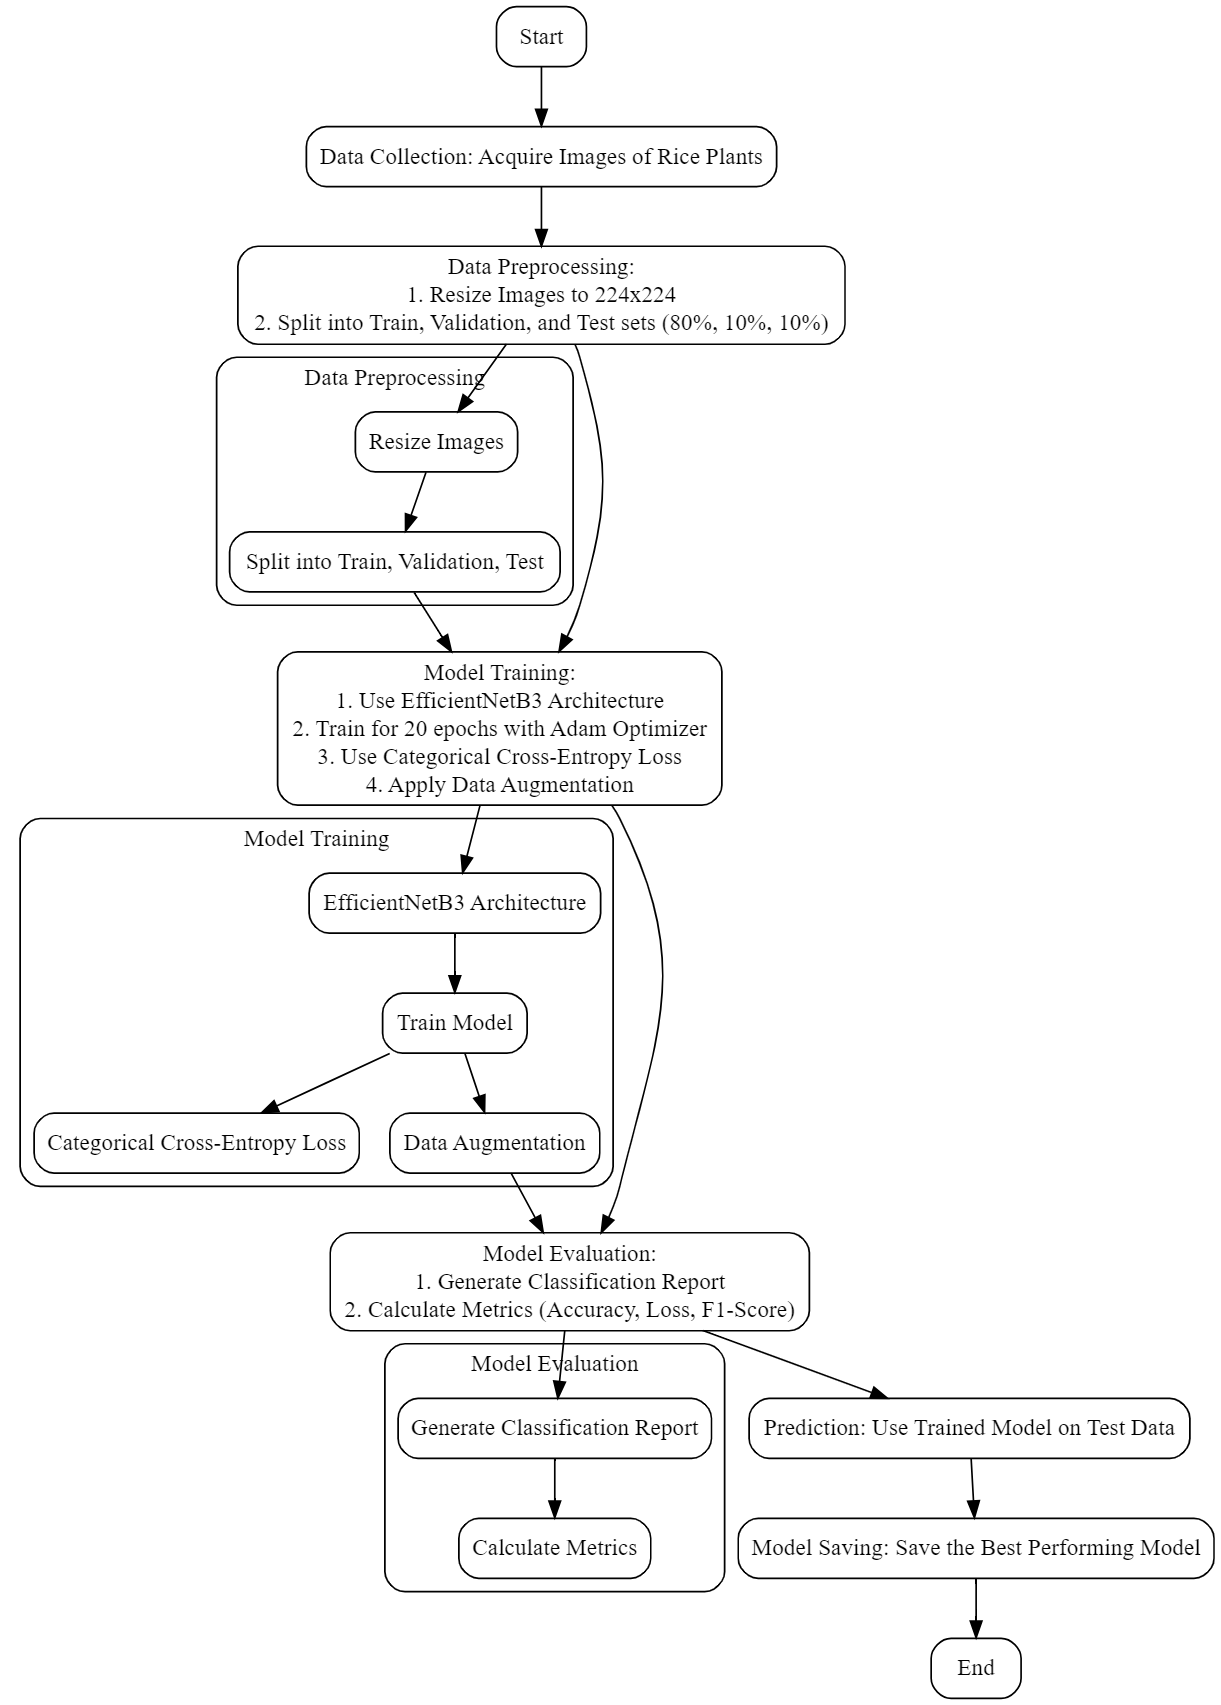
\includegraphics[width=\linewidth]{fig1.png}}
    \caption{Workflow Chart.}
    \label{fig1}
\end{figure}

\subsection{Data Preparation}

\begin{figure}[H]
    \centerline{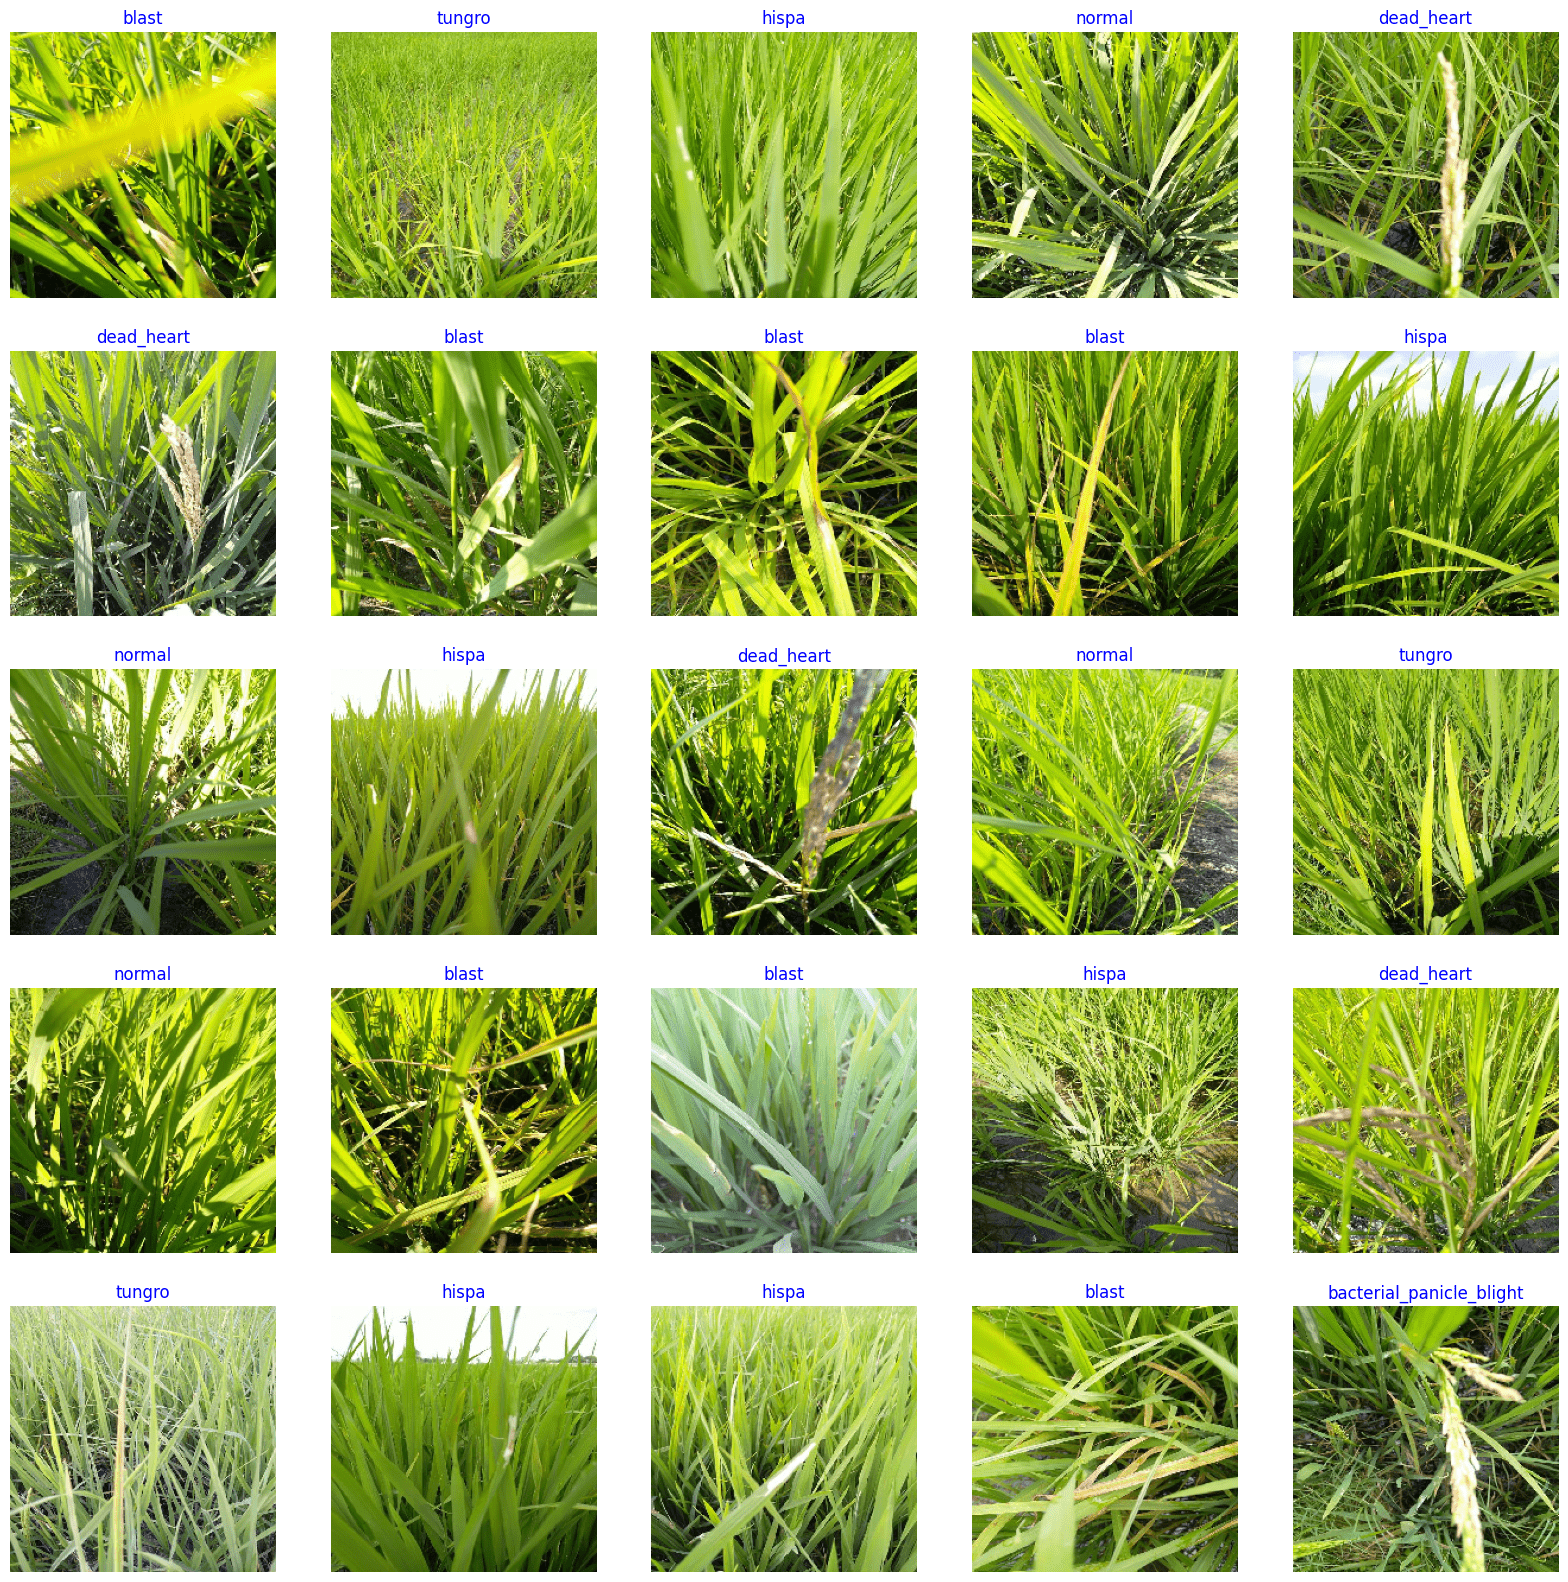
\includegraphics[width=\linewidth]{fig2.png}}
    \caption{Sample image data from Paddy Doctor Dataset.}
    \label{fig2}
\end{figure}

\begin{itemize}
    \item \textbf{Data Collection} The dataset comprised images of rice plants, categorized into different disease classes. It was collected from Paddy Doctor: Paddy Disease Classification in Kaggle. Figure \ref{fig2} shows a sample of the ised image data.
    \item \textbf{Image Resizing} All images were resized to 224x224 pixels. This standardization ensured consistent input dimensions for the CNN model, improving computational efficiency and facilitating model training.
\end{itemize}

\subsection{Data Splitting and Distribution}
The dataset was split into training, validation, and test sets using a stratified approach to maintain class distribution across each subset. Figure \ref{fig2} shows the data distribution between train, test and validation dataset.
\begin{itemize}
    \item \textbf{Training set} 80\% of the total dataset (8325 images) was allocated for model training.
    \item \textbf{Validation set} 10\% of the total dataset (1041 images) was reserved for hyperparameter tuning and model evaluation during training.
    \item \textbf{Test set} The remaining 10\% (1041 images) was kept separate for final model evaluation and performance assessment.
\end{itemize}

\begin{figure}[H]
    \centerline{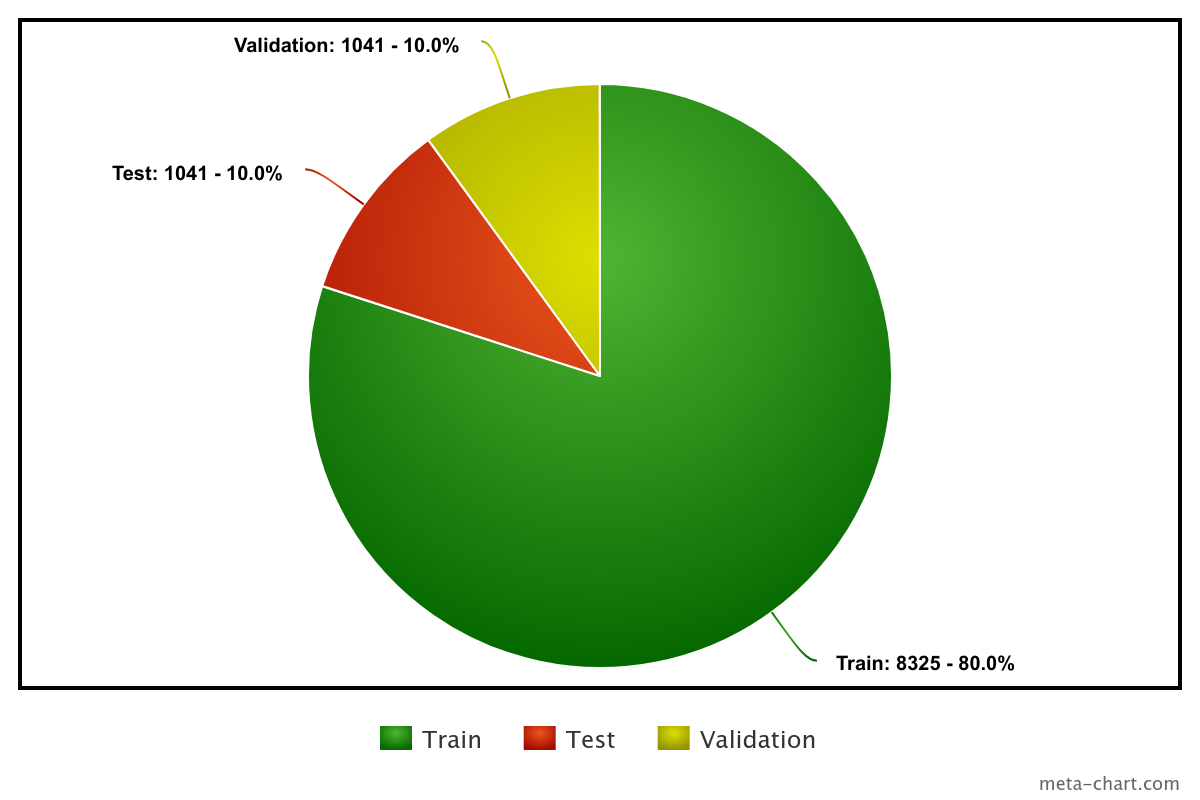
\includegraphics[width=\linewidth]{fig3.png}}
    \caption{Data was distribution proportionality between the three sets.}
    \label{fig3}
\end{figure}

\subsection{Model Training}
\begin{itemize}
    \item \textbf{Model Architecture} The EfficientNetB3 architecture was chosen due to its efficiency and performance on image classification tasks. EfficientNetB3 is part of the EfficientNet family, employing a compound scaling method to optimize both depth and width of the network. It consists of 7 convolutional layers followed by a fully connected layer, with 3.1 million trainable parameters.
    \item \textbf{Training Parameters} The model was trained for 20 epochs using the Adam optimizer with a learning rate of 0.001.
    \item \textbf{Loss Function} The Categorical Cross-Entropy was used as the loss function to measure the difference between predicted and true class labels.
\end{itemize}

\subsection{Model Evaluation and Metrics}
\begin{itemize}
    \item \textbf{Classification Reports} After training, a comprehensive classification report was generated to assess the model's performance across each class. This report included metrics like precision, recall, F1-score, and support.
    \item \textbf{Performance Metrics} Key metrics like accuracy, loss, and F1-score were calculated for both the training and validation sets to monitor model convergence and prevent overfitting.
\end{itemize}

\subsection{Prediction and Model Saving}
\begin{itemize}
    \item \textbf{Test Predictions} The trained model was used to predict the class labels for the unseen test set.
    \item \textbf{Model Saving} The final trained model with the best performance on the validation set was saved for future use and deployment.
\end{itemize}


\section{Results and Discussion}
\subsection{Training and Validation Performance}
To evaluate the performance of the CNN model trained on EfficientNetB3, we monitored both the training and validation loss and accuracy over 20 epochs. The results are depicted in Figure \ref{fig4}.

\begin{figure}[H]
    \centerline{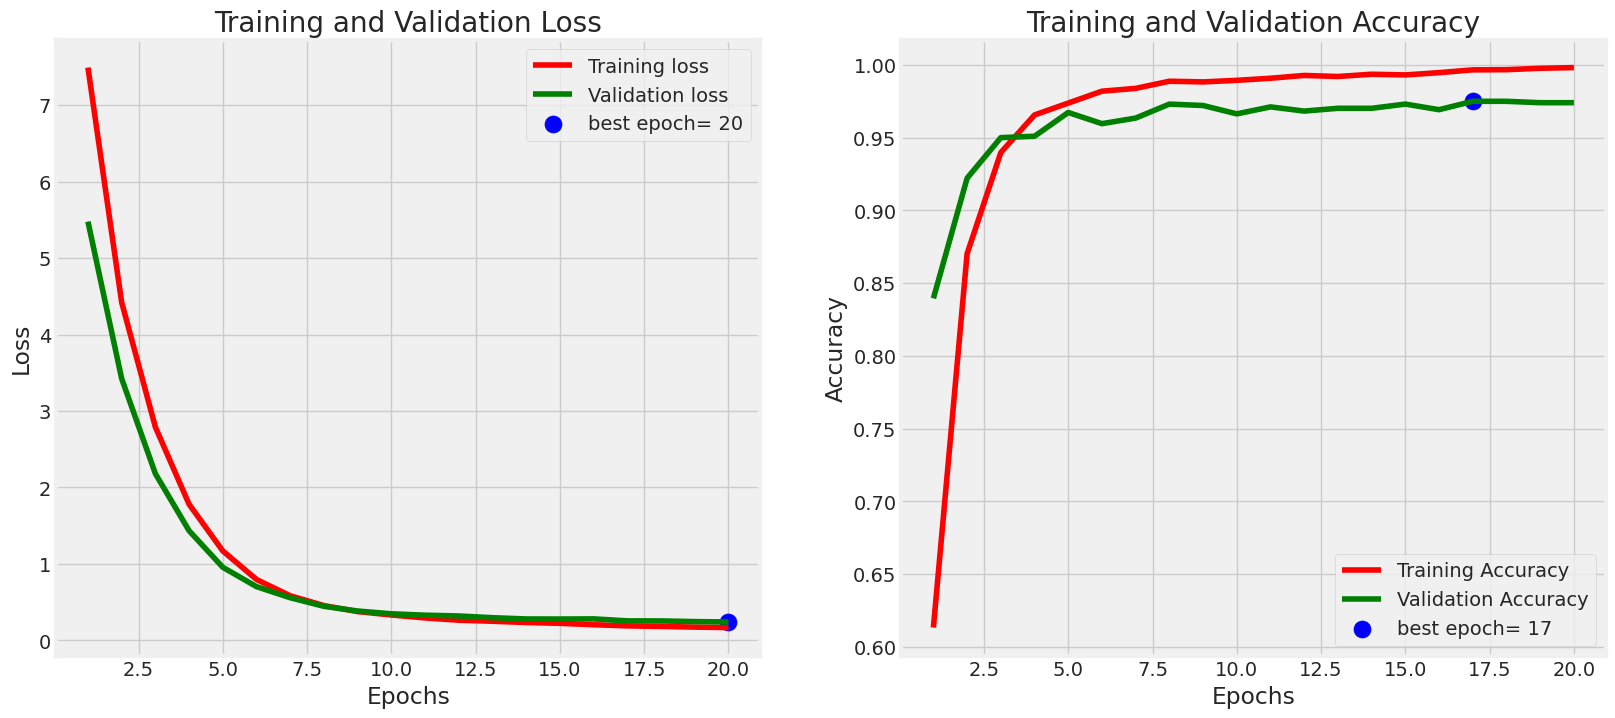
\includegraphics[width=\linewidth]{fig4.png}}
    \caption{Training and Validation Loss and Accuracy.}
    \label{fig4}
\end{figure}

The training loss and validation loss curves exhibit a steady decline over the epochs, with both converging to low values. The training loss starts at approximately 7.5 and drops to below 0.5 by the 20th epoch, while the validation loss starts higher than the training loss but follows a similar decreasing trend, stabilizing around 0.5. This indicates that the model is effectively learning and generalizing well to the validation set.
For accuracy, the training accuracy begins at around 60\% and quickly improves, reaching nearly 100\% by the 20th epoch. The validation accuracy follows closely, starting at around 65\% and stabilizing around 97\%. The best validation accuracy is observed at the 17th epoch, indicating minimal overfitting and good generalization.

\subsection{Loss and Accuracy Calculations}
\subsubsection{Training and Validation Loss}
The loss for each sample is calculated using the categorical cross-entropy loss function, which is given by:

\[
\text{Loss} = -\sum_{i=1}^{N} y_i \log(\hat{y}_i)
\]

where $y_i$ is the true label, $\hat{y}_i$ is the predicted probability for class $i$, and $N$ is the number of classes.
The average loss over all samples in a batch is used to update the model weights during training. The training loss is calculated over the training dataset, and the validation loss is calculated over the validation dataset.

\subsubsection{Training and Validation Accuracy}
Accuracy is calculated as the ratio of correctly predicted samples to the total number of samples, defined as:

\[
    \text{Accuracy} = \frac{\text{Number of Correct Predictions}}{\text{Total Number of Predictions}}
\]

The model's accuracy is computed for both the training and validation datasets. High training accuracy alongside high validation accuracy indicates that the model generalizes well to unseen data.

\subsection{Confusion Matrix Analysis}
The confusion matrix Figure \ref{fig5} provides a detailed breakdown of the model's performance across different classes.

\begin{figure}[H]
    \centerline{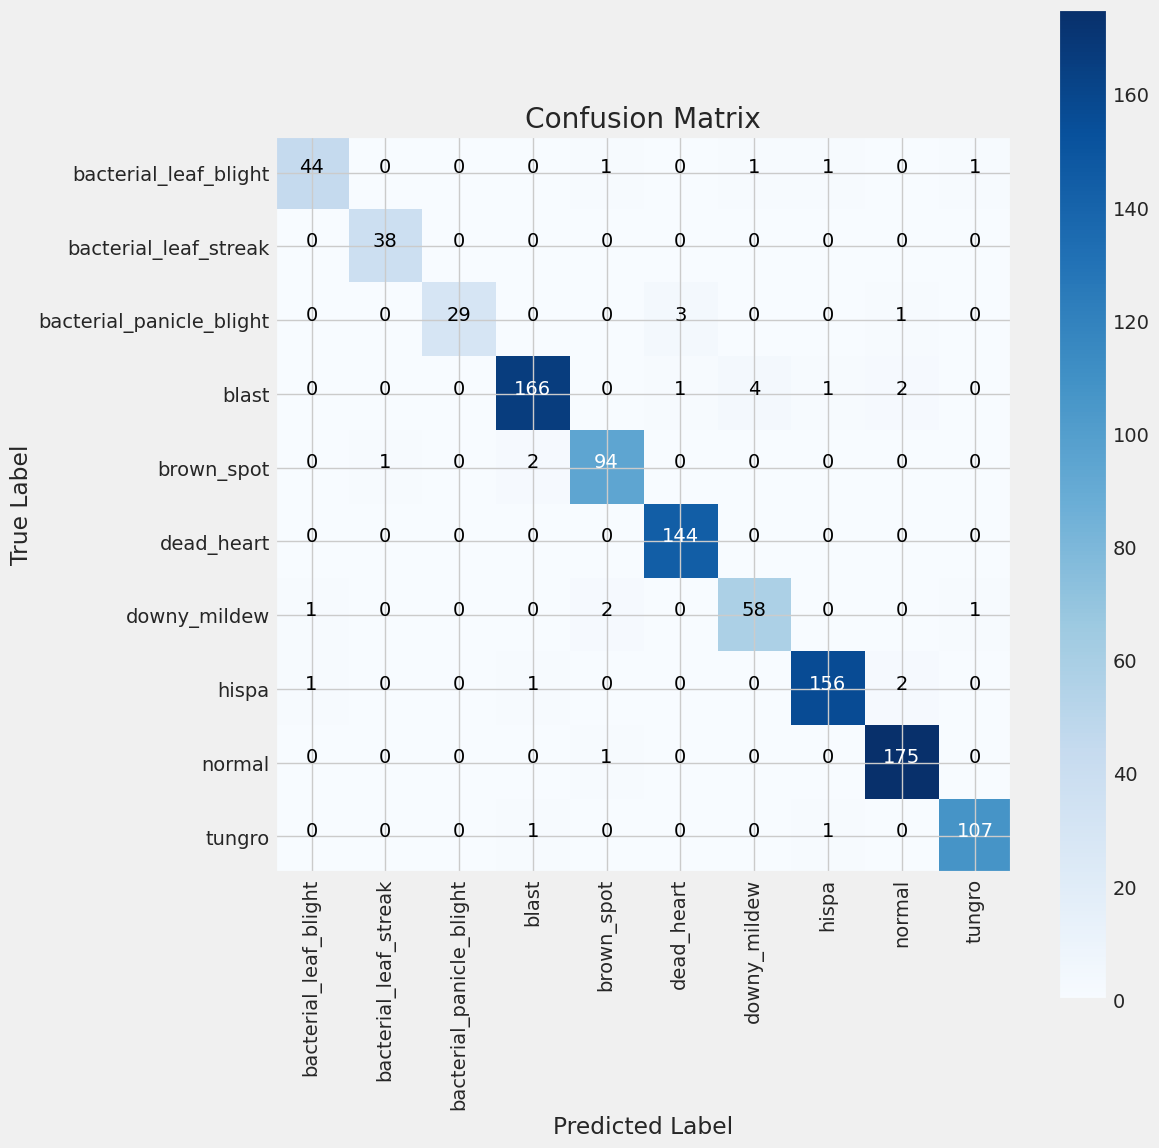
\includegraphics[width=\linewidth]{fig5.png}}
    \caption{Confusion Matrix.}
    \label{fig5}
\end{figure}

The confusion matrix shows the number of correct and incorrect predictions for each class. The diagonal elements represent the true positives (correct predictions), while the off-diagonal elements represent false positives and false negatives.
From the confusion matrix, it is evident that the model performs exceptionally well for most classes, with high true positive rates and low misclassification rates. For example, the class blast has 166 correct predictions and only a few misclassifications. Similarly, the normal class has 175 correct predictions, indicating a high degree of accuracy.
However, some classes exhibit slight confusion, such as bacterial\_panicle\_blight being misclassified as blast (3 instances). This suggests that while the model is highly accurate, there is still room for improvement in distinguishing between certain classes.

\subsection{Classification Report}
Table \ref{tab:classification_report} The classification report, derived from the confusion matrix, provides additional metrics such as precision, recall, and F1-score for each class. Here is a summary of the classification report:

\begin{table}[H]
    \centering
    \captionsetup{skip=5pt}
    \begin{tabular}{lcccc}
    \hline
    \textbf{Class}                  & \textbf{Precision} & \textbf{Recall} & \textbf{F1-score} & \textbf{Support} \\ \hline
    bacterial\_leaf\_blight        & 0.94               & 0.88            & 0.91              & 50               \\
    bacterial\_leaf\_streak        & 0.95               & 1.00            & 0.97              & 38               \\
    bacterial\_panicle\_blight     & 0.91               & 0.83            & 0.87              & 35               \\
    blast                          & 0.97               & 0.95            & 0.96              & 174              \\
    brown\_spot                    & 0.92               & 0.96            & 0.94              & 98               \\
    dead\_heart                    & 1.00               & 1.00            & 1.00              & 144              \\
    downy\_mildew                  & 0.90               & 0.91            & 0.91              & 64               \\
    hispa                          & 0.97               & 0.97            & 0.97              & 161              \\
    normal                         & 0.98               & 0.99            & 0.98              & 177              \\
    tungro                         & 0.97               & 0.99            & 0.98              & 108              \\ \hline
    \textbf{Accuracy}               &                    &                 & 0.96              & 1049             \\
    \textbf{Macro avg}              & 0.95               & 0.95            & 0.95              & 1049             \\
    \textbf{Weighted avg}           & 0.96               & 0.96            & 0.96              & 1049             \\ \hline
    \end{tabular}
    \caption{Classification Report}
    \label{tab:classification_report}
\end{table}

\begin{itemize}
    \item Precision measures the accuracy of positive predictions, defined as 
    \[
    \text{Precision} = \frac{TP}{TP + FP}
    \]
    \item Recall measures the ability to identify all positive instances, defined as 
    \[
    \text{Recall} = \frac{TP}{TP + FN}
    \]
    \item F1-score is the harmonic mean of precision and recall, defined as 
    \[
    \text{F1-score} = 2 \cdot \frac{\text{Precision} \cdot \text{Recall}}{\text{Precision} + \text{Recall}}
    \]
\end{itemize}

The high precision and recall across most classes indicate that the model is both accurate and reliable in its predictions.

\subsection{In-Depth Analysis}
The results demonstrate that the CNN model trained on EfficientNetB3 achieves high accuracy and generalization capability. The convergence of training and validation loss curves and the minimal gap between training and validation accuracy suggest that the model is neither underfitting nor overfitting.

\subsubsection{Overfitting and Underfitting Analysis:}
\begin{itemize}
    \item \textbf{Overfitting} occurs when the model performs well on training data but poorly on validation data. This is not observed here, as the training and validation curves are closely aligned.
    \item \textbf{Underfitting} occurs when the model performs poorly on both training and validation data. This is also not observed, as both training and validation accuracies are high.
\end{itemize}

\subsubsection{Confusion Matrix Insights:}
\begin{itemize}
    \item \textbf{High True Positives} Most classes exhibit a high number of true positives, indicating that the model correctly identifies the majority of samples.
    \item \textbf{False Positives and False Negatives} There are some misclassifications (false positives and false negatives), particularly between classes with similar visual features (e.g., bacterial\_panicle\_blight and blast). This suggests the need for more distinct feature learning.
\end{itemize}

\subsubsection{Precision, Recall, and F1-Score:}
\begin{itemize}
    \item \textbf{High Precision and Recall} High values indicate that the model is effective in both detecting true positives and avoiding false positives.
    \item \textbf{Balanced F1-Scores} High F1-scores across classes indicate a good balance between precision and recall.
\end{itemize}

\section{Conclusion}
In conclusion this research paper investigates the use of various pre-trained Convolutional Neural Network (CNN) models to detect diseases in paddy leaves.

The authors collected images of paddy leaves with different diseases, applied standard image processing techniques, and trained the EfficientNetB3 model on these images. They evaluated the model based on accuracy, precision, recall, and F1-score. The results showed that the EfficientNetB3 model achieved a remarkable accuracy of 96\%.

The study found high precision and recall for most disease classes, meaning the model was generally accurate in its predictions. Specifically, for bacterial leaf blight, the model achieved a precision of 0.94, recall of 0.88, and F1-score of 0.91. For bacterial leaf streak, it achieved a precision of 0.95, recall of 1.00, and F1-score of 0.97. The precision, recall, and F1-scores for other diseases like blast, brown spot, dead heart, downy mildew, hispa, normal, and tungro were similarly high, with most exceeding 0.90. The overall accuracy was 96\%, with macro and weighted averages of precision, recall, and F1-scores all around 0.95 and 0.96, respectively.

The authors demonstrates that the EfficientNetB3 model is highly effective for detecting paddy leaf diseases. This can help farmers diagnose diseases more quickly and accurately, potentially leading to better crop yields and improved food security. The success of the EfficientNetB3 model underscores the critical role of deep learning in advancing agricultural practices and enhancing the productivity and stability of paddy production.

\subsection{Discussion}
The results demonstrate that the CNN model trained on EfficientNetB3 achieves high accuracy and generalization capability. The convergence of training and validation loss curves and the minimal gap between training and validation accuracy suggest that the model is neither underfitting nor overfitting.

The confusion matrix and classification report further confirm the model's robust performance, with high precision, recall, and F1-scores across all classes. Some minor misclassifications indicate potential areas for improvement, possibly through more extensive data augmentation or tuning of hyperparameters.

Overall, the model's performance is highly satisfactory, making it a reliable tool for the classification of rice diseases. Future work could focus on addressing the slight misclassifications and further optimizing the model for even higher accuracy and robustness. This might include:

\begin{itemize}
    \item Data Augmentation: Enhance the dataset with more diverse samples to improve model robustness.
    \item Hyperparameter Tuning: Fine-tune learning rates, batch sizes, and other parameters to achieve better performance.
    \item Model Architecture Improvements: Experiment with different CNN architectures or ensemble methods to further enhance accuracy.
\end{itemize}

\begin{thebibliography}{00}
\bibitem{b1} Deep Learning Approach for Paddy Field Detection Using Labeled Aerial Images: The Case of Detecting and Staging Paddy Fields in Central and Southern Taiwan. Remote sensing,  doi: 10.3390/rs15143575
\bibitem{b2} Salman, Qadri., Hadia, Bibi., Muhammad, Imran, Sharif., Francesco, Marinello. (2023). Comparing Inception V3, VGG 16, VGG 19, CNN, and ResNet 50: A Case Study on Early Detection of a Rice Disease. Agronomy, doi: 10.3390/agronomy13061633
\bibitem{b3} Dingju, Zhu., Jianbin, Tan., Kai, Leung, Yung., Andrew, W., H., Ip. (2023). Crop Disease Identification by Fusing Multiscale Convolution and Vision Transformer. Sensors,  doi: 10.3390/s23136015
\bibitem{b4} V., Senthil, Kumar., M.K., Jaganathan., Abhishek, Viswanathan., M., Umamaheswari., J., C., Vignesh. (2023). Rice leaf disease detection based on bidirectional feature attention pyramid network with YOLO v5 model. Environmental research communications,  doi: 10.1088/2515-7620/acdece
\bibitem{b5} Leong, Qi, Yang., Xiaoyun, Yu., Shaoping, Zhang., Huanhuan, Zhang., Shuang, Xu., Hu, Long., Yingwen, Zhu. (2023). Stacking-based and improved convolutional neural network: a new approach in rice leaf disease identification. Frontiers in Plant Science,  doi: 10.3389/fpls.2023.1165940
\bibitem{b6} A High-Quality Rice Leaf Disease Image Data Augmentation Method Based on a Dual GAN. IEEE Access,  doi: 10.1109/access.2023.3251098
\bibitem{b7} Alam, T.S., Jowthi, C.B. \& Pathak, A. Comparing pre-trained models for efficient leaf disease detection: a study on custom CNN. Journal of Electrical Systems and Inf Technol 11, 12 (2024). https://doi.org/10.1186/s43067-024-00137-1
\bibitem{b8} Soo, Jun, Wei., Dimas, Firmanda, Al, Riza., Hermawan, Eko, Nugroho. (2022). Comparative study on the performance of deep learning implementation in the edge computing: Case study on the plant leaf disease identification. Journal of agriculture and food research,  doi: 10.1016/j.jafr.2022.100389
\bibitem{b9} Chakraborty, A., Chakraborty, A., Sobhan, A., \& Pathak, A. Deep Learning for Precision Agriculture: Detecting Tomato Leaf Diseases with VGG-16 Model. International Journal of Computer Applications, 975, 8887.
\bibitem{b10} Ghazanfar, Latif., Sherif, Elmeligy, Abdelhamid., Roxane, Elias, Mallouhy., Jaafar, Alghazo., Z., A., Kazimi. (2022). Deep Learning Utilization in Agriculture: Detection of Rice Plant Diseases Using an Improved CNN Model. Plants,  doi: 10.3390/plants11172230
\end{thebibliography}


\end{document}
